\chapter{随机近似与随机梯度下降}
\label{ch:rl-sa}

% ════════════════════════════════════════════════════════════════
%  忠实转录自《强化学习的数学原理》(赵世钰) 第6章「随机近似算法」
%  原原本本、逐字保全；以源页 PDF (p121--p144) 为完整性与正确性基准。
%  图分层：6.1 导航图→弃用(nav-drop)；6.2 黑盒示意→TikZ；
%          6.3 / 6.4 / 6.5 收敛曲线/散点/热图→raster includegraphics。
% ════════════════════════════════════════════════════════════════

% TODO[nav-drop]: 图6.1「本章在全书中的位置」(images/91deef...jpg) 为 Zhao 全书导航图，按约定弃用。

上一章介绍了基于蒙特卡罗的无需模型的强化学习算法，下一章（第7章）将介绍另一种无需模型的强化学习算法——时序差分。然而，在开始介绍下一章的内容之前，我们需要按下暂停键，先学习本章关于随机近似算法的内容。为什么要这么做呢？我们到目前为止学习的算法都是非增量式的（non-incremental）。然而，时序差分算法是增量式的（incremental），它与我们之前学习过的算法看起来非常不同。许多读者在第一次看到时序差分算法时会有很多问题，例如这些算法为什么设计成这个样子、它们为什么能有效工作等。为了让大家能更容易地理解时序差分算法，我们在本章先来介绍随机近似算法。时序差分算法可以被视为特殊的随机近似算法；经典的随机梯度下降也是特殊的随机近似算法。

\section{启发示例：期望值估计}
\label{sec:rl-sa-mean}

期望值估计问题已经在上一章讨论过一次。下面我们从另一个角度再次研究这个问题，并且介绍如何用“增量式”的方法解决这个问题。

考虑一个随机变量 $X$，它取值于有限集 $\mathcal{X}$。我们的目标是估计期望值 $\mathbb{E}[X]$。假设有一个独立同分布的样本序列 $\{x_i\}_{i=1}^n$。那么 $X$ 的期望值可以通过这些样本的平均值来近似：
\begin{equation}
\mathbb{E}[X] \approx \bar{x} \doteq \frac{1}{n} \sum_{i=1}^{n} x_i.
\label{eq:rl-sa-6-1}
\end{equation}
式\eqref{eq:rl-sa-6-1}就是蒙特卡罗估计的基本思想，并且大数定律告诉我们，当 $n\to\infty$ 时，$\bar{x}\to \mathbb{E}[X]$。这些已经在第5章介绍过了。

有两种方法可以计算平均值 $\bar{x}$。第一种是非增量式的（non-incremental）：首先收集所有样本，然后计算平均值。这种方法的缺点是如果样本数量很大，可能需要等待很久才能把所有样本收集完毕。第二种是增量式的（incremental）。具体来说，令
\begin{equation}
w_{k+1} \doteq \frac{1}{k} \sum_{i=1}^{k} x_i, \quad k = 1, 2, \dots
\end{equation}
类似地
\begin{equation}
w_k = \frac{1}{k-1} \sum_{i=1}^{k-1} x_i, \quad k = 2, 3, \dots
\end{equation}
实际上，$w_{k+1}$ 可以用 $w_k$ 表示：
\begin{equation}
w_{k+1} = \frac{1}{k} \sum_{i=1}^{k} x_i = \frac{1}{k} \left( \sum_{i=1}^{k-1} x_i + x_k \right) = \frac{1}{k} \big( (k-1) w_k + x_k \big) = w_k - \frac{1}{k} (w_k - x_k).
\end{equation}
因此，我们得到如下增量式算法：
\begin{equation}
w_{k+1} = w_k - \frac{1}{k} (w_k - x_k).
\label{eq:rl-sa-6-2}
\end{equation}
该算法可以以增量的方式计算均值 $\bar{x}$。

为了验证该算法，我们可以计算出 $k = 1, 2, \ldots$ 次迭代的结果：
\begin{equation}
\begin{aligned}
w_1 &= x_1, \\
w_2 &= w_1 - \frac{1}{1} (w_1 - x_1) = x_1, \\
w_3 &= w_2 - \frac{1}{2} (w_2 - x_2) = x_1 - \frac{1}{2} (x_1 - x_2) = \frac{1}{2} (x_1 + x_2), \\
w_4 &= w_3 - \frac{1}{3} (w_3 - x_3) = \frac{1}{3} (x_1 + x_2 + x_3), \\
&\;\;\vdots
\end{aligned}
\end{equation}
\begin{equation}
w_{k+1} = \frac{1}{k} \sum_{i=1}^{k} x_i.
\label{eq:rl-sa-6-3}
\end{equation}
可以看出，由这个增量式算法得到的 $w_{k+1}$ 确实是 $\{x_i\}_{i=1}^k$ 的平均值。这里 $w_1 = x_1$ 是初始值。

算法\eqref{eq:rl-sa-6-2}的优势在于，每次接收到一个样本时，平均值就可以立即计算出来，进而近似 $\mathbb{E}[X]$。由于样本不足，开始时近似可能不够准确，不过这总比没有好。随着获取更多样本，估计的准确度会逐渐提高。此外，我们也可以定义 $w_{k+1} = \frac{1}{1+k}\sum_{i=1}^{k+1}x_i$ 和 $w_k = \frac{1}{k}\sum_{i=1}^{k}x_i$。在这种情况下，相应的迭代算法是 $w_{k+1} = w_k - \frac{1}{1+k}(w_k - x_{k+1})$。最后，我们可以把\eqref{eq:rl-sa-6-2}推广得到一个更一般化的算法：
\begin{equation}
w_{k+1} = w_k - \alpha_k (w_k - x_k).
\label{eq:rl-sa-6-4}
\end{equation}
与\eqref{eq:rl-sa-6-2}相比，上式将系数 $1/k$ 替换为 $\alpha_k > 0$。由于这里 $\alpha_k$ 的表达式未给出，因此无法像\eqref{eq:rl-sa-6-3}中那样给出 $w_k$ 的显式表达式，不过我们仍然可以分析其收敛性，具体将在下一节介绍。

算法\eqref{eq:rl-sa-6-4}非常重要，且在本章经常出现。我们在第7章将看到时序差分算法与\eqref{eq:rl-sa-6-4}非常类似，这也是我们介绍该算法的主要原因，理解该算法将有助于理解时序差分算法。

\section{罗宾斯-门罗算法}
\label{sec:rl-sa-rm}

随机近似（stochastic approximation）指的是一大类用于求解方程或者优化问题的随机迭代算法\textsuperscript{[24]}。罗宾斯-门罗（Robbins-Monro，RM）算法是随机近似领域的开创性工作\textsuperscript{[24--27]}。\pz{原书引文献编号 [24]--[32]、[7,8] 等，本笔记暂沿用原编号以 \texttt{textsuperscript} 标注，待统一并入 refs.bib}著名的随机梯度下降算法是 RM 算法的一种特殊形式（参见\cref{sec:rl-sa-sgd}）。

下面介绍 RM 算法。假设我们想要求解如下方程：
\begin{equation}
g(w) = 0,
\end{equation}
其中 $w \in \mathbb{R}$ 是未知变量，$g: \mathbb{R} \to \mathbb{R}$ 是一个函数。许多问题都可以描述为上面的方程求根问题。例如，如果 $J(w)$ 是一个需要优化的目标函数，这个优化问题可以转换为求解方程 $g(w) \doteq \nabla_w J(w) = 0$。另外，如果方程右边有一个常数，例如 $f(w) = c$，此时仍然可以转化为上式的形式，例如 $g(w) \doteq f(w) - c = 0$。

如果 $g$ 表达式是已知的，那么有很多数值算法可以用来求解 $g(w) = 0$。然而，我们面临的问题是函数 $g$ 的表达式是未知的，我们只知道该函数的输入和输出。具体来说，当输入 $w$ 时，我们可以观测其输出值，而且该输出值可能还包含观测噪声：
\begin{equation}
\tilde{g}(w, \eta) = g(w) + \eta,
\end{equation}
其中 $\eta \in \mathbb{R}$ 是观测噪声，而且可能不是高斯分布的。总而言之，该函数是一个黑盒系统，例如是一个人工神经网络（\cref{fig:rl-sa-blackbox}）。此时，我们就可以用 RM 算法来求解。

\begin{figure}[H]
\centering
\begin{tikzpicture}[>=Stealth, font=\small]
  \node[draw, rounded corners, minimum width=26mm, minimum height=14mm,
        fill=main!8, draw=main!60!black, align=center] (box) {$g(w)$\\[-1pt]\scriptsize 黑盒系统};
  \node[left=14mm of box] (in) {$w$};
  \node[right=16mm of box] (out) {$\tilde{g} = g(w) + \eta$};
  \draw[->, thick] (in) -- (box);
  \draw[->, thick] (box) -- (out);
  \node[above=2mm of box, font=\scriptsize] {含噪声};
\end{tikzpicture}
\caption{函数 $g(w)$ 的示意图：输入是 $w$，含噪声的输出是 $\tilde{g}$。}
\label{fig:rl-sa-blackbox}
\end{figure}

求解 $g(w) = 0$ 的 RM 算法是
\begin{equation}
w_{k+1} = w_k - a_k \tilde{g}(w_k, \eta_k), \qquad k = 1, 2, 3, \ldots
\label{eq:rl-sa-6-5}
\end{equation}
其中 $w_k$ 是第 $k$ 次方程解的估计值，$\tilde{g}(w_k, \eta_k)$ 是输入 $w_k$ 后输出的观测值，$a_k$ 是一个正系数。可以看到，RM 算法不需要关于函数表达式的任何信息，而仅需要输入和输出。

在分析该算法的理论性质之前，我们先看一个直观的例子以更好地理解 RM 算法。考虑方程 $g(w) = w^3 - 5$，其真实的解是 $w = 5^{1/3} \approx 1.71$。现在我们只能观测输入 $w$ 和输出 $\tilde{g}(w) = g(w) + \eta$，其中假设 $\eta$ 是独立同分布的，并且服从均值为 0 且标准差为 1 的正态分布。初始值是 $w_1 = 0$，系数是 $a_k = 1/k$。$w_k$ 的演变过程如\cref{fig:rl-sa-w3}所示。尽管观测值受到 $\eta_k$ 的噪声干扰，但估计的 $w_k$ 仍然可以收敛到真实的解。值得指出的是，如果初始值 $w_1$ 选择的不合适，RM 算法可能会发散，这是由函数 $g(w) = w^3 - 5$ 的一些性质决定的。RM 算法的收敛性将在下一节详细介绍。

\begin{figure}[H]
\centering
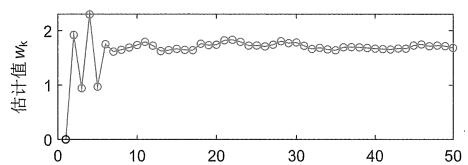
\includegraphics[width=0.46\textwidth]{figures/rl/5230491c874047fe2329b74a6306400f2f370dafec37fd706c10567934452b62.jpg}\hfill
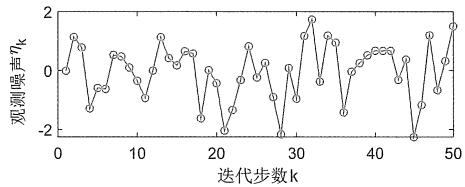
\includegraphics[width=0.46\textwidth]{figures/rl/b710b47085b45ebc2f1481fee99af9f35307b946d7d862ecc0594f77aa923b40.jpg}
\caption{用 RM 算法求解 $g(w) = w^3 - 5$ 的过程。}
\label{fig:rl-sa-w3}
\end{figure}

\subsection{收敛性质}
\label{sec:rl-sa-rm-conv}

为什么\eqref{eq:rl-sa-6-5}中的 RM 算法能找到 $g(w) = 0$ 的根呢？下面通过一个例子来直观地解释，之后再提供严格的收敛性分析。

在\cref{fig:rl-sa-tanh}所示的例子中，$g(w) = \tanh(w - 1)$。因为这个例子很简单，可以知道 $g(w) = 0$ 的真实解是 $w^* = 1$。下面看 RM 算法能否成功得到这个解。选取为 $w_1 = 3$ 和 $a_k = 1/k$。为了更好地说明收敛的原因，我们考虑最简单的没有观测噪声的情况：$\eta_k \equiv 0$，即 $\tilde{g}(w_k, \eta_k) = g(w_k)$。此时，RM 算法变为 $w_{k+1} = w_k - a_k g(w_k)$。\cref{fig:rl-sa-tanh}展示了由该算法生成的 $\{w_k\}$。可以看出，$w_k$ 最终成功收敛到 $w^* = 1$。这个简单的例子能从直观上解释为什么 RM 算法会收敛。

\begin{figure}[H]
\centering
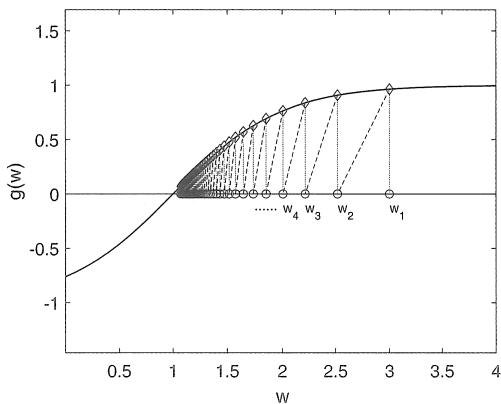
\includegraphics[width=0.62\textwidth]{figures/rl/21f4f539b26e694ccbaa5dfb9c15f604cb5f5bec56ec8115819b3e9404adbeef.jpg}
\caption{用 RM 算法求解 $g(w) = \tanh(w - 1) = 0$ 的过程。}
\label{fig:rl-sa-tanh}
\end{figure}

\begin{itemize}
  \item 当 $w_k > w^*$ 时，有 $g(w_k) > 0$。此时 $w_{k+1} = w_k - a_k g(w_k) < w_k$。如果 $a_k$ 足够小，我们有 $w^* < w_{k+1} < w_k$。因此 $w_{k+1}$ 比 $w_k$ 更接近 $w^*$。
  \item 当 $w_k < w^*$ 时，有 $g(w_k) < 0$。此时 $w_{k+1} = w_k - a_k g(w_k) > w_k$。如果 $a_k$ 足够小，我们有 $w^* > w_{k+1} > w_k$。因此 $w_{k+1}$ 比 $w_k$ 更接近 $w^*$。
\end{itemize}

总而言之，因为 $w_{k+1}$ 总是比 $w_k$ 更接近于 $w^*$，所以从直观上可以知道 $w_k$ 收敛于 $w^*$。

上面的例子很简单，并没有考虑观测误差。在一般情况下，当有观测误差时，下面的定理给出了严格的收敛性结果。

\begin{theorem}[罗宾斯-门罗定理]\label{thm:rl-sa-rm}
在\eqref{eq:rl-sa-6-5}的 RM 算法中，如果下面三个条件全部成立：
\begin{enumerate}
  \item[(a)] 存在两个常数 $c_1, c_2 > 0$，使得 $0 < c_1 \leqslant \nabla_w g(w) \leqslant c_2$ 对于所有的 $w$ 成立；
  \item[(b)] $\sum_{k=1}^{\infty} a_k = \infty$ 且 $\sum_{k=1}^{\infty} a_k^2 < \infty$；
  \item[(c)] $\mathbb{E}[\eta_k | \mathcal{H}_k] = 0$ 且 $\mathbb{E}[\eta_k^2 | \mathcal{H}_k] < \infty$，其中 $\mathcal{H}_k = \{w_k, w_{k-1}, \ldots\}$；
\end{enumerate}
那么 $w_k$ 几乎必然收敛到 $g(w^*) = 0$ 的根 $w^*$。
\end{theorem}

罗宾斯-门罗定理（简称 RM 定理）涉及几乎必然（almost surely）收敛的概念，相关概念在附录 B 有详细介绍。这个定理的证明并非一蹴而就，我们将在\cref{sec:rl-sa-dvor-rm}给出详细证明。下面首先讨论如何理解该定理中的三个条件。

\begin{itemize}
  \item 在条件 (a) 中，$0 < c_1 \leqslant \nabla_w g(w)$ 要求 $g(w)$ 是一个单调递增的函数。这个条件确保 $g(w) = 0$ 的根存在并且是唯一的。

  如果 $g(w)$ 是一个目标函数 $J(w)$ 的梯度，即 $g(w) \doteq \nabla_w J(w)$，那么 $c_1 \leqslant \nabla_w g(w)$ 等价于 $c_1 \leqslant \nabla_w^2 J(w)$，这意味着 $J(w)$ 是凸的（convex），这是在优化问题中经常采用的假设，也说明该条件是比较宽松的。此外，如果 $g(w)$ 是单调递减的，我们可以简单地将 $-g(w)$ 视为一个新的单调递增的函数。

  不等式 $\nabla_w g(w) \leqslant c_2$ 表明 $g(w)$ 的梯度不能趋于无穷。$g(w) = \tanh(w - 1)$ 是满足这个条件的，但是前面提到过的一个例子 $g(w) = w^3 - 5$ 则不满足这个条件。因此，当我们用 RM 算法求解 $g(w) = w^3 - 5 = 0$ 时，需要选取合适的初始值，否则可能发散。

  \item 条件 (b) 是关于 $a_k$ 的，我们经常在强化学习算法中看到类似的条件。其中 $\sum_{k=1}^{\infty} a_k^2 < \infty$ 意味着 $\lim_{n \to \infty} \sum_{k=1}^{n} a_k^2$ 是有上界的，这要求 $a_k$ 随着 $k \to \infty$ 收敛到 0。条件 $\sum_{k=1}^{\infty} a_k = \infty$ 意味着 $\lim_{n \to \infty} \sum_{k=1}^{n} a_k$ 是无限大的，这要求 $a_k$ 不能太快地收敛到 0。这些条件很有意思，稍后将做详细分析。

  \item 条件 (c) 是关于噪声 $\eta_k$ 的，它并不要求观测误差 $\eta_k$ 是高斯分布的。该条件成立的一个重要特例是 $\{\eta_k\}$ 是一个独立同分布的随机序列，因此满足 $\mathbb{E}[\eta_k] = 0$ 且 $\mathbb{E}[\eta_k^2] < \infty$。此时，因为 $\eta_k$ 与 $\mathcal{H}_k$ 是独立的，所以 $\mathbb{E}[\eta_k | \mathcal{H}_k] = \mathbb{E}[\eta_k] = 0$ 且 $\mathbb{E}[\eta_k^2 | \mathcal{H}_k] = \mathbb{E}[\eta_k^2]$。
\end{itemize}

下面更加细致地讨论\cref{thm:rl-sa-rm}中的条件 (b)，即关于 $a_k$ 的条件。

\paragraph{为什么条件 (b) 对 RM 算法的收敛是必要的？}
当然，我们稍后给出的定理的严格证明可以很自然地回答这个问题。不过，我们先简要介绍一下其基本思想。

第一，条件 $\sum_{k=1}^{\infty} a_k^2 < \infty$ 要求随着 $k \to \infty$ 时 $a_k \to 0$。这个条件为什么重要呢？由于
\begin{equation}
w_{k+1} - w_k = -a_k \tilde{g}(w_k, \eta_k),
\end{equation}
如果 $a_k \to 0$，那么 $a_k \tilde{g}(w_k, \eta_k) \to 0$（假设 $\tilde{g}(w_k, \eta_k)$ 总是有界的）。因此，$w_{k+1} - w_k \to 0$，即当 $k \to \infty$ 时 $w_{k+1}$ 与 $w_k$ 非常接近。反过来说，如果 $a_k$ 不会收敛到 0，那么 $w_{k+1}$ 可能不会与 $w_k$ 很近，因此 $w_k$ 会一直波动而无法收敛。

第二，条件 $\sum_{k=1}^{\infty} a_k = \infty$ 表明 $a_k$ 不能太快收敛到 0。这个条件为什么重要呢？如果我们把 RM 算法的每一步写出来，可得 $w_2 - w_1 = -a_1 \tilde{g}(w_1, \eta_1)$，$w_3 - w_2 = -a_2 \tilde{g}(w_2, \eta_2)$，$w_4 - w_3 = -a_3 \tilde{g}(w_3, \eta_3)$，$\ldots$。把这些式子两边分别相加可以得到
\begin{equation}
w_1 - w_\infty = \sum_{k=1}^{\infty} a_k \tilde{g}(w_k, \eta_k).
\end{equation}
我们用反证法。假设 $\sum_{k=1}^{\infty} a_k < \infty$，进而 $\left| \sum_{k=1}^{\infty} a_k \tilde{g}(w_k, \eta_k) \right|$ 也是有上界的，令 $b$ 表示这个上界。因此可以得到
\begin{equation}
\left| w_1 - w_\infty \right| = \left| \sum_{k=1}^{\infty} a_k \tilde{g}(w_k, \eta_k) \right| \leqslant b.
\label{eq:rl-sa-6-6}
\end{equation}
此时，如果我们选取的初始值 $w_1$ 离方程的解 $w^*$ 很远，以至于 $|w_1 - w^*| > b$，那么\eqref{eq:rl-sa-6-6}告诉我们 $w_\infty = w^*$ 是不可能的，所以在这种情况下 RM 算法无法找到 $w^*$。因此，为了确保选取任意初始值时 RM 算法都能收敛，条件 $\sum_{k=1}^{\infty} a_k = \infty$ 是必需的。

\paragraph{什么样的序列 $\{a_k\}_{k=1}^{\infty}$ 满足 $\sum_{k=1}^{\infty} a_k = \infty$ 且 $\sum_{k=1}^{\infty} a_k^2 < \infty$ 呢？}
一个典型的序列是
\begin{equation}
a_k = \frac{1}{k}.
\end{equation}
一方面，$\{a_k = 1/k\}$ 满足
\begin{equation}
\lim_{n \to \infty} \left( \sum_{k=1}^{n} \frac{1}{k} - \ln n \right) = \kappa,
\end{equation}
其中 $\kappa \approx 0.577$ 称为欧拉-马歇罗尼常数（Euler-Mascheroni constant）或欧拉常数（Euler's constant）\textsuperscript{[28]}。上式表明 $\sum_{k=1}^{n} \frac{1}{k}$ 与 $\ln n$ 在 $n \to \infty$ 时的误差是一个很小的常数。由于当 $n \to \infty$ 时 $\ln n \to \infty$，因此
\begin{equation}
\sum_{k=1}^{\infty} \frac{1}{k} = \infty.
\end{equation}
实际上，$\sum_{k=1}^{n} \frac{1}{k}$ 在数论中有一个专门的名字：调和数（harmonic number）。更多信息可参见\textsuperscript{[29]}。

另一方面，$\{a_k = 1/k\}$ 满足
\begin{equation}
\sum_{k=1}^{\infty} \frac{1}{k^2} = \frac{\pi^2}{6} < \infty.
\end{equation}
为什么上式成立呢？求解 $\sum_{k=1}^{\infty} \frac{1}{k^2}$ 的值的问题被称为巴塞尔问题（Basel problem），更多信息可参见\textsuperscript{[30]}。

综上所述，序列 $\{a_k = 1/k\}$ 满足\cref{thm:rl-sa-rm}中的条件 (b)。值得注意的是，对条件 (b) 稍加修改（例如 $a_k = 1/(k+1)$ 或 $a_k = 10/k$）仍然可以满足条件 (b)。

值得一提的是，$a_k$ 在实际中常常会被选择为一个小的正数。此时，条件 $\sum_{k=1}^{\infty} a_k = \infty$ 仍然成立，但是条件 $\sum_{k=1}^{\infty} a_k^2 < \infty$ 不再成立。这样选择 $a_k$ 的原因是它能够很好地利用后面（$k$ 比较大时）得到的样本。否则，如果 $a_k$ 逐渐收敛到 0，那么当 $k$ 较大时，得到的数据对 $w_k$ 的影响已经微乎其微了。实际上，当 $a_k$ 恒等于一个正数时，算法仍然可以在某种意义上收敛，详情参见文献\textsuperscript{[24]}（第 1.5 节）。实际中，我们之所以希望 $k$ 比较大时样本数据仍然有效，其本质原因是这可以应对时变系统（例如函数 $g(w)$ 随时间缓慢变化）。

\subsection{在期望值估计问题中的应用}
\label{sec:rl-sa-rm-mean}

\cref{sec:rl-sa-mean}已经对增量式期望值估计算法有过讨论。我们先简要回忆一下。式\eqref{eq:rl-sa-6-4}给出了一个迭代算法：$w_{k+1} = w_k + \alpha_k (x_k - w_k)$。当 $\alpha_k = 1/k$ 时，可以得到 $w_{k+1}$ 的解析表达式为 $w_{k+1} = \frac{1}{k}\sum_{i=1}^{k} x_i$。然而，当 $\alpha_k$ 取一般值时，我们将无法得到 $w_{k+1}$ 的解析表达式。此时这个算法仍然能求解期望值估计问题吗？

下面展示算法\eqref{eq:rl-sa-6-4}实际上是一个特殊的 RM 算法，因此其收敛性也可以得到保证。具体来说，定义如下函数：
\begin{equation}
g(w) \doteq w - \mathbb{E}[X].
\end{equation}
此时，求解期望值 $\mathbb{E}[X]$ 的问题可以转换成求解方程 $g(w) = 0$ 的问题。由于我们能得到 $X$ 的随机样本 $x$，对任意给定的 $w$ 值，我们能获得的带噪声的观测值为 $\tilde{g} \doteq w - x$。

$\tilde{g}$ 可以进一步写成
\begin{equation}
\begin{aligned}
\tilde{g}(w, \eta) &= w - x \\
&= w - x + \mathbb{E}[X] - \mathbb{E}[X] \\
&= (w - \mathbb{E}[X]) + (\mathbb{E}[X] - x) \doteq g(w) + \eta,
\end{aligned}
\end{equation}
其中 $\eta \doteq \mathbb{E}[X] - x$。这样我们就把期望值估计的问题转换为一个可以用 RM 算法求解的问题。相应的 RM 算法是
\begin{equation}
w_{k+1} = w_k - \alpha_k \tilde{g}(w_k, \eta_k) = w_k - \alpha_k (w_k - x_k).
\end{equation}
上式正是\eqref{eq:rl-sa-6-4}中的算法。根据\cref{thm:rl-sa-rm}，如果 $\sum_{k=1}^{\infty} \alpha_k = \infty$ 且 $\sum_{k=1}^{\infty} \alpha_k^2 < \infty$，并且 $\{x_k\}$ 是独立同分布的，那么 $w_k$ 将几乎必然收敛到 $\mathbb{E}[X]$。值得一提的是，该收敛性质不依赖于 $X$ 的分布假设。

\section{Dvoretzky 定理}
\label{sec:rl-sa-dvor}

下面证明\cref{thm:rl-sa-rm}从而证明 RM 算法的收敛性。为此，我们首先介绍一个重要的结果：Dvoretzky 定理\textsuperscript{[31,\,32]}。这是随机近似领域的一个经典结果，该结果可以用来分析 RM 算法以及许多强化学习算法的收敛性。

值得提醒大家的是，本节有较多的数学内容。如果大家对随机近似算法的收敛分析感兴趣，推荐阅读本节；否则可以跳过这一节，并不会影响后续章节的学习。

\begin{theorem}[Dvoretzky 定理]\label{thm:rl-sa-dvor}
考虑如下的随机过程：
\begin{equation}
\Delta_{k+1} = (1 - \alpha_k) \Delta_k + \beta_k \eta_k,
\end{equation}
其中 $\{\alpha_k\}_{k=1}^{\infty}, \{\beta_k\}_{k=1}^{\infty}, \{\eta_k\}_{k=1}^{\infty}$ 是随机序列，且 $\alpha_k \geqslant 0, \beta_k \geqslant 0$。如果以下条件成立，那么 $\Delta_k$ 将几乎必然收敛到 0：
\begin{enumerate}
  \item[(a)] $\sum_{k=1}^{\infty} \alpha_k = \infty$，$\sum_{k=1}^{\infty} \alpha_k^2 < \infty$，$\sum_{k=1}^{\infty} \beta_k^2 < \infty$ 一致几乎必然成立；
  \item[(b)] $\mathbb{E}[\eta_k | \mathcal{H}_k] = 0$ 并且 $\mathbb{E}[\eta_k^2 | \mathcal{H}_k] \leqslant C$ 几乎必然成立。
\end{enumerate}
其中 $\mathcal{H}_k = \{\Delta_k, \Delta_{k-1}, \dots, \eta_{k-1}, \dots, \alpha_{k-1}, \dots, \beta_{k-1}, \dots\}$。
\end{theorem}

在证明这个定理之前，我们首先解释该定理中的一些条件。

\begin{itemize}
  \item 在 RM 算法中，序列 $\{a_k\}$ 是确定性的。在 Dvoretzky 定理中，$\{\alpha_k\}$ 和 $\{\beta_k\}$ 可以是依赖 $\mathcal{H}_k$ 的随机变量，这更加一般化，可以处理 $\alpha_k$ 和 $\beta_k$ 是 $\Delta_k$ 的函数的情况。

  Dvoretzky 定理的第一个条件涉及“一致几乎必然”（uniformly almost surely），这是因为当 $\alpha_k$ 和 $\beta_k$ 是随机变量时，其极限的定义必须是在随机意义上的。第二个条件也提到了“几乎必然”。这是因为 $\mathcal{H}_k$ 是随机变量，此时条件期望 $\mathbb{E}[\eta_k | \mathcal{H}_k]$ 和 $\mathbb{E}[\eta_k^2 | \mathcal{H}_k]$ 也是随机变量，其定义是在“几乎必然”意义上的。详情可参见附录 B。

  \item \cref{thm:rl-sa-dvor}的表述与\textsuperscript{[32]}略有不同：其第一个条件不要求 $\sum_{k=1}^{\infty} \beta_k = \infty$，这是因为当 $\sum_{k=1}^{\infty} \beta_k < \infty$，特别是在极端情况下 $\beta_k = 0$ 时，序列仍然可以收敛。
\end{itemize}

\subsection{Dvoretzky 定理的证明}
\label{sec:rl-sa-dvor-proof}

Dvoretzky 定理的证明有多种方法，其原始证明在 1956 年给出\textsuperscript{[31]}。下面给出一种基于准鞅（quasi-martingale）的证明。利用准鞅的收敛性性质，Dvoretzky 定理的证明会更加容易。关于准鞅的更多信息可参见附录 C。

\begin{proof}[证明 Dvoretzky 定理]
设 $h_k \doteq \Delta_k^2$。那么，
\begin{equation}
\begin{aligned}
h_{k+1} - h_k &= \Delta_{k+1}^2 - \Delta_k^2 \\
&= (\Delta_{k+1} - \Delta_k)(\Delta_{k+1} + \Delta_k) \\
&= (-\alpha_k \Delta_k + \beta_k \eta_k) \big[ (2 - \alpha_k) \Delta_k + \beta_k \eta_k \big] \\
&= -\alpha_k (2 - \alpha_k) \Delta_k^2 + \beta_k^2 \eta_k^2 + 2 (1 - \alpha_k) \beta_k \eta_k \Delta_k.
\end{aligned}
\end{equation}
对上式两边取期望可得
\begin{equation}
\mathbb{E}[h_{k+1} - h_k | \mathcal{H}_k] = \mathbb{E}[-\alpha_k (2 - \alpha_k) \Delta_k^2 | \mathcal{H}_k] + \mathbb{E}[\beta_k^2 \eta_k^2 | \mathcal{H}_k] + \mathbb{E}[2 (1 - \alpha_k) \beta_k \eta_k \Delta_k | \mathcal{H}_k].
\label{eq:rl-sa-6-7}
\end{equation}
首先，由于 $\Delta_k$ 被包含在 $\mathcal{H}_k$ 中，因此可以从条件期望中提取出来（参见 Lemma~B.1 的性质 (e)）。其次，假设 $\alpha_k, \beta_k$ 可由 $\mathcal{H}_k$ 确定，此假设在 $\{\alpha_k\}$ 和 $\{\beta_k\}$ 是确定性序列或者是 $\Delta_k$ 的函数时是成立的。此时，它们也可以从条件期望中提取出来。这样\eqref{eq:rl-sa-6-7}就变成了
\begin{equation}
\mathbb{E}[h_{k+1} - h_k | \mathcal{H}_k] = -\alpha_k (2 - \alpha_k) \Delta_k^2 + \beta_k^2 \mathbb{E}[\eta_k^2 | \mathcal{H}_k] + 2 (1 - \alpha_k) \beta_k \Delta_k \mathbb{E}[\eta_k | \mathcal{H}_k].
\label{eq:rl-sa-6-8}
\end{equation}
对于第一项，因为 $\sum_{k=1}^{\infty} \alpha_k^2 < \infty$ 可以推出 $\alpha_k \to 0$ 是几乎必然的，所以存在一个有限的 $n$ 使得几乎必然对所有 $k \geqslant n$ 有 $\alpha_k \leqslant 1$。不失一般性，我们只考虑 $k \geqslant n$ 即 $\alpha_k \leqslant 1$ 的情况。此时，$-\alpha_k (2 - \alpha_k) \Delta_k^2 \leqslant 0$。对于第二项，根据定理中的条件，我们有 $\beta_k^2 \mathbb{E}[\eta_k^2 | \mathcal{H}_k] \leqslant \beta_k^2 C$。第三项等于 0，这可以由定理中的条件 $\mathbb{E}[\eta_k | \mathcal{H}_k] = 0$ 得到。因此，\eqref{eq:rl-sa-6-8}变为
\begin{equation}
\mathbb{E}[h_{k+1} - h_k | \mathcal{H}_k] = -\alpha_k (2 - \alpha_k) \Delta_k^2 + \beta_k^2 \mathbb{E}[\eta_k^2 | \mathcal{H}_k] \leqslant \beta_k^2 C,
\label{eq:rl-sa-6-9}
\end{equation}
即
\begin{equation}
\sum_{k=1}^{\infty} \mathbb{E}[h_{k+1} - h_k | \mathcal{H}_k] \leqslant \sum_{k=1}^{\infty} \beta_k^2 C < \infty.
\end{equation}
上式中的第二个小于号是因为 $\sum_{k=1}^{\infty} \beta_k^2 < \infty$。基于附录 C 中的准鞅收敛定理，我们得出 $h_k$ 是几乎必然收敛的。

下面确定 $\Delta_k$ 会收敛到什么值。根据\eqref{eq:rl-sa-6-9}可得
\begin{equation}
\sum_{k=1}^{\infty} \alpha_k (2 - \alpha_k) \Delta_k^2 = \sum_{k=1}^{\infty} \beta_k^2 \mathbb{E}[\eta_k^2 | \mathcal{H}_k] - \sum_{k=1}^{\infty} \mathbb{E}[h_{k+1} - h_k | \mathcal{H}_k].
\end{equation}
根据定理中的条件，上式右侧第一项是有界的，第二项也是有界的，这是因为 $h_k$ 是收敛的，从而 $h_{k+1} - h_k$ 是可求和的。因此，等式左边的 $\sum_{k=1}^{\infty} \alpha_k (2 - \alpha_k) \Delta_k^2$ 也是有界的。由于我们考虑的是 $\alpha_k \leqslant 1$ 的情况，可得
\begin{equation}
\infty > \sum_{k=1}^{\infty} \alpha_k (2 - \alpha_k) \Delta_k^2 \geqslant \sum_{k=1}^{\infty} \alpha_k \Delta_k^2 \geqslant 0.
\end{equation}
因此 $\sum_{k=1}^{\infty} \alpha_k \Delta_k^2$ 是有界的。由于 $\sum_{k=1}^{\infty} \alpha_k = \infty$，可得 $\Delta_k \to 0$ 是几乎必然的。
\end{proof}

\subsection{应用于分析期望值估计算法}
\label{sec:rl-sa-dvor-mean}

对于期望值估计算法 $w_{k+1} = w_k + \alpha_k (x_k - w_k)$，我们已经在\cref{sec:rl-sa-rm-mean}使用 RM 定理分析了其收敛性。下面展示其收敛性也可以直接通过 Dvoretzky 定理来证明。

\begin{proof}
设 $w^* = \mathbb{E}[X]$。期望值估计算法 $w_{k+1} = w_k + \alpha_k (x_k - w_k)$ 可以重写为
\begin{equation}
w_{k+1} - w^* = w_k - w^* + \alpha_k (x_k - w^* + w^* - w_k).
\end{equation}
令 $\Delta \doteq w - w^*$。那么上式可写成
\begin{equation}
\begin{aligned}
\Delta_{k+1} &= \Delta_k + \alpha_k (x_k - w^* - \Delta_k) \\
&= (1 - \alpha_k) \Delta_k + \alpha_k \underbrace{(x_k - w^*)}_{\eta_k}.
\end{aligned}
\end{equation}
由于 $\{x_k\}$ 是独立同分布的，我们有 $\mathbb{E}[x_k | \mathcal{H}_k] = \mathbb{E}[x_k] = w^*$。因此，$\mathbb{E}[\eta_k | \mathcal{H}_k] = \mathbb{E}[x_k - w^* | \mathcal{H}_k] = 0$，并且 $\mathbb{E}[\eta_k^2 | \mathcal{H}_k] = \mathbb{E}[x_k^2 | \mathcal{H}_k] - (w^*)^2 = \mathbb{E}[x_k^2] - (w^*)^2$ 在 $x_k$ 的方差有限的情况下是有界的。根据 Dvoretzky 定理，可知 $\Delta_k$ 几乎必然收敛至 0，因此 $w_k$ 几乎必然收敛至 $w^* = \mathbb{E}[X]$。
\end{proof}

\subsection{应用于证明罗宾斯-门罗定理}
\label{sec:rl-sa-dvor-rm}

之前我们在给出罗宾斯-门罗定理（RM 定理）时并没有给出其证明，下面使用 Dvoretzky 定理来证明 RM 定理。

\begin{proof}[证明 RM 定理]
RM 算法旨在求解 $g(w) = 0$。假设其真实解是 $w^*$，即 $g(w^*) = 0$。RM 算法的表达式为
\begin{equation}
\begin{aligned}
w_{k+1} &= w_k - a_k \tilde{g}(w_k, \eta_k) \\
&= w_k - a_k [ g(w_k) + \eta_k ].
\end{aligned}
\end{equation}
在上式两边同减去 $w^*$ 可得
\begin{equation}
w_{k+1} - w^* = w_k - w^* - a_k \left[ g(w_k) - g(w^*) + \eta_k \right].
\end{equation}
根据中值定理\textsuperscript{[7,\,8]}可得 $g(w_k) - g(w^*) = \nabla_w g(w_k') (w_k - w^*)$，其中 $w_k' \in [w_k, w^*]$。如果进一步设 $\Delta_k \doteq w_k - w^*$，则上述方程变为
\begin{equation}
\begin{aligned}
\Delta_{k+1} &= \Delta_k - a_k [ \nabla_w g(w_k') (w_k - w^*) + \eta_k ] \\
&= \Delta_k - a_k \nabla_w g(w_k') \Delta_k + a_k (-\eta_k) \\
&= \big[ 1 - \underbrace{a_k \nabla_w g(w_k')}_{\alpha_k} \big] \Delta_k + a_k (-\eta_k).
\end{aligned}
\end{equation}
首先，RM 定理中的条件 $c_1 \leqslant \nabla_w g(w) \leqslant c_2$ 表明 $\nabla_w g(w)$ 是有界的。此外，由定理中的条件 $\sum_{k=1}^{\infty} a_k = \infty$ 和 $\sum_{k=1}^{\infty} a_k^2 < \infty$，可得 $\sum_{k=1}^{\infty} \alpha_k = \infty$ 和 $\sum_{k=1}^{\infty} \alpha_k^2 < \infty$。因此，Dvoretzky 定理中的条件都是满足的，进而可知 $\Delta_k$ 几乎必然收敛到 0。
\end{proof}

通过证明 RM 定理，我们知道了 Dvoretzky 定理是一个更加一般化的定理。例如，虽然上述证明中的 $\alpha_k$ 是一个依赖于 $w_k$ 的随机序列，而并不是一个确定性序列，但是 Dvoretzky 定理仍然适用。

\subsection{Dvoretzky 定理的推广}
\label{sec:rl-sa-dvor-ext}

下面我们进一步推广 Dvoretzky 定理，从而得到一个能够处理多变量的更加一般化的定理，可用于分析诸如 Q-learning 等随机迭代算法的收敛性。

\begin{theorem}\label{thm:rl-sa-dvor-ext}
给定一个有限实数集合 $\mathcal{S}$。对 $s \in \mathcal{S}$ 有如下随机过程：
\begin{equation}
\Delta_{k+1}(s) = (1 - \alpha_k(s)) \Delta_k(s) + \beta_k(s) \eta_k(s).
\end{equation}
如果对于所有 $s \in \mathcal{S}$ 下面的条件都成立，那么 $\Delta_k(s)$ 几乎必然收敛到 0：
\begin{enumerate}
  \item[(a)] $\sum_k \alpha_k(s) = \infty$，$\sum_k \alpha_k^2(s) < \infty$，$\sum_k \beta_k^2(s) < \infty$，并且 $\mathbb{E}[\beta_k(s) | \mathcal{H}_k] \leqslant \mathbb{E}[\alpha_k(s) | \mathcal{H}_k]$ 一致几乎必然成立；
  \item[(b)] $\| \mathbb{E}[\eta_k(s) | \mathcal{H}_k] \|_\infty \leqslant \gamma \| \Delta_k \|_\infty$，其中 $\gamma \in (0, 1)$；
  \item[(c)] $\operatorname{var}[\eta_k(s) | \mathcal{H}_k] \leqslant C (1 + \| \Delta_k(s) \|_\infty)^2$，这里 $C$ 是一个常数。
\end{enumerate}
其中 $\mathcal{H}_k = \{\Delta_k, \Delta_{k-1}, \ldots, \eta_{k-1}, \ldots, \alpha_{k-1}, \ldots, \beta_{k-1}, \ldots\}$ 代表历史信息，$\| \cdot \|_\infty$ 代表最大范数。
\end{theorem}

该定理可以基于 Dvoretzky 定理得到证明，详细信息可参见\textsuperscript{[32]}。下面给出一些关于该定理的解释。

首先澄清定理中的一些符号。变量 $s$ 可以被视为一个索引。在强化学习中，它可以是状态的索引。最大范数 $\| \cdot \|_\infty$ 是定义在一个集合上的。例如，$\| \mathbb{E}[\eta_k(s) | \mathcal{H}_k] \|_\infty \doteq \max_{s \in \mathcal{S}} |\mathbb{E}[\eta_k(s) | \mathcal{H}_k]|$，$\| \Delta_k(s) \|_\infty \doteq \max_{s \in \mathcal{S}} |\Delta_k(s)|$。这与向量的 $L^\infty$ 范数类似但不完全相同。

该定理比 Dvoretzky 定理更加一般化。首先，它通过使用最大范数 $\| \cdot \|_\infty$ 可以处理多个变量，即证明多个变量对应的随机过程都收敛。这对于处理涉及多个状态的强化学习问题很重要。其次，Dvoretzky 定理要求 $\mathbb{E}[\eta_k(s) | \mathcal{H}_k] = 0$ 且 $\operatorname{var}[\eta_k(s) | \mathcal{H}_k] \leqslant C$，而该定理仅要求期望和方差由误差 $\Delta_k$ 界定。

值得注意的是，$\Delta(s)$ 的收敛性要求定理中的条件对每一个 $s \in \mathcal{S}$ 都是成立的。因此，在应用此定理来证明强化学习算法的收敛性时，我们需要证明该定理中的条件对每个状态（或状态-动作对）都是成立的。

\section{随机梯度下降}
\label{sec:rl-sa-sgd}

本节将介绍在机器学习领域广为使用的随机梯度下降（stochastic gradient descent, SGD）算法。而且我们将会知道：随机梯度下降算法是一种特殊的 RM 算法，而前面介绍过的期望值估计算法是一种特殊的随机梯度下降算法。

考虑如下优化问题：
\begin{equation}
\min_w J(w) = \mathbb{E}[f(w, X)],
\label{eq:rl-sa-6-10}
\end{equation}
其中 $w$ 是需要优化的参数，$X$ 是一个随机变量，这里期望值是针对 $X$ 的。这里 $w$ 和 $X$ 可以是标量或者向量，而函数 $f(\cdot)$ 是一个标量。

解决\eqref{eq:rl-sa-6-10}的常见方法是梯度下降（gradient descent）。由于 $\mathbb{E}[f(w, X)]$ 的梯度是 $\nabla_w \mathbb{E}[f(w, X)] = \mathbb{E}[\nabla_w f(w, X)]$，相应的梯度下降算法是
\begin{equation}
w_{k+1} = w_k - \alpha_k \nabla_w J(w_k) = w_k - \alpha_k \mathbb{E}[\nabla_w f(w_k, X)].
\label{eq:rl-sa-6-11}
\end{equation}
梯度下降算法在一些条件下（例如 $f$ 是凸函数）可以找到全局最优解 $w^*$。关于梯度下降算法的更多信息可参见附录 D。

梯度下降算法需要依赖于期望值 $\mathbb{E}[\nabla_w f(w_k, X)]$。我们知道有两种获取期望值的方法（见第 5.1 节）。第一种方法是基于模型的方法，即利用 $X$ 的概率分布和期望值的定义直接计算，然而 $X$ 的概率分布可能是难以得到的；第二种方法是基于数据的方法，即利用独立同分布的样本 $\{x_i\}_{i=1}^n$ 来计算：
\begin{equation}
\mathbb{E}[\nabla_w f(w_k, X)] \approx \frac{1}{n} \sum_{i=1}^{n} \nabla_w f(w_k, x_i).
\end{equation}
此时\eqref{eq:rl-sa-6-11}变为
\begin{equation}
w_{k+1} = w_k - \frac{\alpha_k}{n} \sum_{i=1}^{n} \nabla_w f(w_k, x_i).
\label{eq:rl-sa-6-12}
\end{equation}
算法\eqref{eq:rl-sa-6-12}的问题在于它在每次迭代中都需要所有样本。如果样本是逐个得到的，则可以用下面的算法：
\begin{equation}
w_{k+1} = w_k - \alpha_k \nabla_w f(w_k, x_k).
\label{eq:rl-sa-6-13}
\end{equation}
其中 $x_k$ 是在时刻 $k$ 得到的样本。上式就是著名的随机梯度下降算法，它之所以被称为随机梯度下降，是因为它用一个基于单个随机样本得到的随机梯度 $\nabla_w f(w_k, x_k)$ 来替换梯度下降算法中的真实梯度 $\mathbb{E}[\nabla_w f(w_k, X)]$。

由于随机梯度 $\nabla_w f(w_k, x_k)$ 不等于真实梯度 $\mathbb{E}[\nabla_w f(w, X)]$，那么替换后该算法能否确保当 $k \to \infty$ 时 $w_k \to w^*$ 呢？答案是可以的。下面我们先给出一个直观的解释，之后在\cref{sec:rl-sa-sgd-conv}给出严格的证明。具体来说，随机梯度可以重新写成
\begin{equation}
\begin{aligned}
\nabla_w f(w_k, x_k) &= \mathbb{E}[\nabla_w f(w_k, X)] + \Big( \nabla_w f(w_k, x_k) - \mathbb{E}[\nabla_w f(w_k, X)] \Big) \\
&\doteq \mathbb{E}[\nabla_w f(w_k, X)] + \eta_k.
\end{aligned}
\end{equation}
上式表明随机梯度等于真实梯度加一个噪声项 $\eta_k$。将该式代入\eqref{eq:rl-sa-6-13}可得
\begin{equation}
w_{k+1} = w_k - \alpha_k \mathbb{E}[\nabla_w f(w_k, X)] - \alpha_k \eta_k.
\end{equation}
因此，随机梯度下降算法与常规的梯度下降算法的差异仅仅是一个噪声项 $\alpha_k \eta_k$。由于 $\{x_k\}$ 是独立同分布的，我们有 $\mathbb{E}_{x_k}[\nabla_w f(w_k, x_k)] = \mathbb{E}_X[\nabla_w f(w_k, X)]$。因此，$\eta_k$ 的期望值等于 0：
\begin{equation}
\mathbb{E}[\eta_k] = \mathbb{E}\left[ \nabla_w f(w_k, x_k) - \mathbb{E}[\nabla_w f(w_k, X)] \right] = \mathbb{E}_{x_k}[\nabla_w f(w_k, x_k)] - \mathbb{E}_X[\nabla_w f(w_k, X)] = 0.
\end{equation}
在直观上，由于噪声的均值等于 0，因此它应该不会对收敛性造成太大的危害。更严格的证明将在\cref{sec:rl-sa-sgd-conv}中给出。

\subsection{应用于期望值估计}
\label{sec:rl-sa-sgd-mean}

下面我们用随机梯度下降算法来解决期望值估计问题，我们将看到前面式\eqref{eq:rl-sa-6-4}给出的期望值估计算法是一个特殊的随机梯度下降算法。

首先，将期望值估计问题描述为一个优化问题：
\begin{equation}
\min_w J(w) = \mathbb{E}\left[ \frac{1}{2} \| w - X \|^2 \right] \doteq \mathbb{E}[f(w, X)],
\label{eq:rl-sa-6-14}
\end{equation}
其中 $f(w, X) \doteq \| w - X \|^2 / 2$，其梯度为 $\nabla_w f(w, X) = w - X$。通过求解 $\nabla_w J(w) = 0$ 可以知道该优化问题的最优解是 $w^* = \mathbb{E}[X]$。因此，该优化问题等价于期望值估计问题。

\begin{itemize}
  \item 用于求解\eqref{eq:rl-sa-6-14}的梯度下降算法是
  \begin{equation}
  \begin{aligned}
  w_{k+1} &= w_k - \alpha_k \nabla_w J(w_k) \\
  &= w_k - \alpha_k \mathbb{E}[\nabla_w f(w_k, X)] \\
  &= w_k - \alpha_k \mathbb{E}[w_k - X].
  \end{aligned}
  \end{equation}
  该梯度下降算法无法直接使用，因为其右侧的 $\mathbb{E}[w_k - X]$ 或 $\mathbb{E}[X]$ 是未知的。实际上，$\mathbb{E}[X]$ 正是我们需要求解的。

  \item 用于求解\eqref{eq:rl-sa-6-14}的随机梯度下降算法是
  \begin{equation}
  w_{k+1} = w_k - \alpha_k \nabla_w f(w_k, x_k) = w_k - \alpha_k (w_k - x_k),
  \end{equation}
  其中 $x_k$ 是在时刻 $k$ 获得的样本。这个随机梯度下降算法与\eqref{eq:rl-sa-6-4}给出的期望值估计算法是一模一样的。因此，\eqref{eq:rl-sa-6-4}是一个用于求解期望值估计的随机梯度下降算法。
\end{itemize}

\subsection{随机梯度下降的收敛模式}
\label{sec:rl-sa-sgd-pattern}

随机梯度下降算法的思想是用随机梯度替代真实梯度。由于随机梯度是随机的，读者可能会问其收敛速度是不是很慢或者很随机。实际上，随机梯度下降算法通常可以高效收敛。一个有趣的模式是：当估计值 $w_k$ 远离最优解 $w^*$ 时，随机梯度下降的收敛与常规梯度下降算法类似；只有当 $w_k$ 接近 $w^*$ 时，随机梯度下降的收敛才会表现出更多的随机性。下面是对这一收敛模式的分析和示例。

\paragraph{分析.}
定义随机梯度与真实梯度之间的相对误差：
\begin{equation}
\delta_k \doteq \frac{| \nabla_w f(w_k, x_k) - \mathbb{E}[\nabla_w f(w_k, X)] |}{| \mathbb{E}[\nabla_w f(w_k, X)] |}.
\end{equation}
简单起见，考虑 $w$ 和 $\nabla_w f(w, x)$ 都是标量的情况。由于 $w^*$ 是最优解，因此有 $\mathbb{E}[\nabla_w f(w^*, X)] = 0$。此时，上式可以重新写为
\begin{equation}
\delta_k = \frac{| \nabla_w f(w_k, x_k) - \mathbb{E}[\nabla_w f(w_k, X)] |}{| \mathbb{E}[\nabla_w f(w_k, X)] - \mathbb{E}[\nabla_w f(w^*, X)] |} = \frac{| \nabla_w f(w_k, x_k) - \mathbb{E}[\nabla_w f(w_k, X)] |}{| \mathbb{E}[\nabla_w^2 f(\tilde{w}_k, X) (w_k - w^*)] |}.
\label{eq:rl-sa-6-15}
\end{equation}
上式中第二个等号是根据中值定理\textsuperscript{[7,\,8]}得出的，其中 $\tilde{w}_k \in [w_k, w^*]$。假设 $f$ 是严格凸的，即对任意 $w$ 和 $X$ 有 $\nabla_w^2 f \geqslant c > 0$。此时\eqref{eq:rl-sa-6-15}的分母变为
\begin{equation}
\begin{aligned}
\left| \mathbb{E}[\nabla_w^2 f(\tilde{w}_k, X) (w_k - w^*)] \right| &= \left| \mathbb{E}[\nabla_w^2 f(\tilde{w}_k, X)] \right| \left| (w_k - w^*) \right| \\
&\geqslant c | w_k - w^* |.
\end{aligned}
\end{equation}
将上述不等式代入\eqref{eq:rl-sa-6-15}中可得
\begin{equation}
\delta_k \leqslant \frac{\left| \overbrace{\nabla_w f(w_k, x_k)}^{\text{随机梯度}} - \overbrace{\mathbb{E}[\nabla_w f(w_k, X)]}^{\text{真实梯度}} \right|}{\underbrace{c | w_k - w^* |}_{\text{估计的绝对误差}}}.
\end{equation}
上式表明了梯度的相对误差 $\delta_k$ 与估计的绝对误差 $|w_k - w^*|$ 呈反比。当 $|w_k - w^*|$ 较大时，$\delta_k$ 较小，此时随机梯度和真实梯度差不多，因此随机梯度下降算法的表现类似于梯度下降算法，进而 $w_k$ 会迅速接近 $w^*$，这是我们希望看到的良好性质。当 $|w_k - w^*|$ 较小时，梯度的相对误差 $\delta_k$ 可能会很大，此时随机梯度下降算法的表现相比梯度下降会有更大的随机性，这是使用随机样本难以避免的问题，可以通过使用更多的数据和较小的学习率来缓解随机性问题。

\paragraph{示例.}
下面我们以期望值估计为例来展示上述的收敛模式。考虑式\eqref{eq:rl-sa-6-14}中的期望值估计问题。当 $w$ 和 $X$ 都是标量时，我们有 $f(w, X) = | w - X |^2 / 2$，进而可得
\begin{equation}
\nabla_w f(w, x_k) = w - x_k,
\end{equation}
\begin{equation}
\mathbb{E}[\nabla_w f(w, x_k)] = w - \mathbb{E}[X] = w - w^*.
\end{equation}
此时可以计算得到梯度的相对误差为
\begin{equation}
\begin{aligned}
\delta_k &= \frac{| \nabla_w f(w_k, x_k) - \mathbb{E}[\nabla_w f(w_k, X)] |}{| \mathbb{E}[\nabla_w f(w_k, X)] |} \\
&= \frac{| (w_k - x_k) - (w_k - \mathbb{E}[X]) |}{| w_k - w^* |} \\
&= \frac{| \mathbb{E}[X] - x_k |}{| w_k - w^* |}.
\end{aligned}
\end{equation}
从上式可知两个有意思的性质。第一，$\delta_k$ 与 $|w_k - w^*|$ 呈反比，这与前面的分析是一致的，即当 $w_k$ 离 $w^*$ 比较远时，随机梯度下降和梯度下降的行为是类似的。第二，$\delta_k$ 与 $|\mathbb{E}[X] - x_k|$ 呈正比，这也是一个有意思的性质。实际上，$|\mathbb{E}[X] - x_k|$ 与 $X$ 的方差有关，这是因为方差的定义是 $\operatorname{var}(X) = \mathbb{E}[(\mathbb{E}[X] - X)^2]$。因此，当方差很小时，$|\mathbb{E}[X] - x_k|$ 的值是比较小的，进而 $\delta_k$ 是比较小的，此时随机梯度下降的行为会更加接近梯度下降算法。

\cref{fig:rl-sa-sgd-mean}给出了一个期望值估计的例子。这里 $X \in \mathbb{R}^2$ 代表一个边长为 20 的正方形区域内的一个随机位置，其分布是均匀的，且其真实期望值在原点。该估计过程依赖于 100 个独立同分布的样本。可以看出，虽然初始估计距离真实值很远，但是随机梯度下降能很快接近原点。当估计值接近原点时，收敛过程会表现出一定的随机性。这些现象与前面的理论分析是一致的。

\begin{figure}[H]
\centering
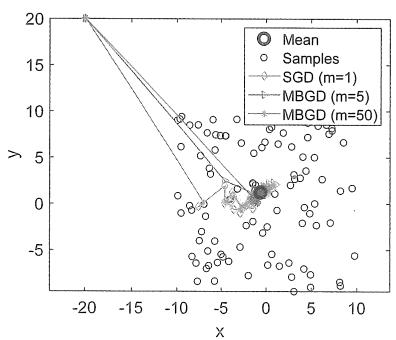
\includegraphics[width=0.46\textwidth]{figures/rl/d5ddbb3ae21e1002cfc02f5427e45a48765e537c55530e33734875edd5d4f399.jpg}\hfill
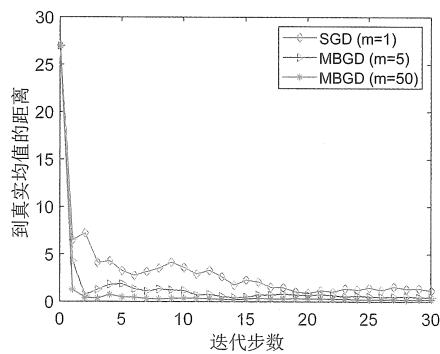
\includegraphics[width=0.46\textwidth]{figures/rl/f279eb45f340bf8d116cf4dfbc42b2b6231b2b98ad8f9637177e65b65c4da03b.jpg}
\caption{对比随机梯度下降和（小批量）梯度下降算法。其中 $\alpha_k = 1/k$。随机变量 $X \in \mathbb{R}^2$ 随机均匀分布在一个以原点为中心、边长为 20 的正方形区域内。估计过程依赖于 100 个独立同分布的样本。}
\label{fig:rl-sa-sgd-mean}
\end{figure}

\subsection{随机梯度下降的另一种描述}
\label{sec:rl-sa-sgd-alt}

式\eqref{eq:rl-sa-6-13}描述的随机梯度下降是涉及随机变量的。有的读者可能会在其他资料中看到另一种描述随机梯度下降算法的方式，而其中并不显式地涉及任何随机变量。

具体来说，考虑一组实数 $\{x_i\}_{i=1}^n$，其中 $x_i$ 并非任何随机变量的样本。这里要解决的优化问题是最小化平均值：
\begin{equation}
\min_w J(w) = \frac{1}{n} \sum_{i=1}^{n} f(w, x_i),
\label{eq:rl-sa-6-16}
\end{equation}
其中 $f(w, x_i)$ 是一个参数化的函数。解决这个问题的梯度下降算法是
\begin{equation}
w_{k+1} = w_k - \alpha_k \nabla_w J(w_k) = w_k - \alpha_k \frac{1}{n} \sum_{i=1}^{n} \nabla_w f(w_k, x_i).
\end{equation}
如果集合 $\{x_i\}_{i=1}^n$ 很大，并且我们每次只能获取一个元素，此时可以用下式来更新 $w_k$
\begin{equation}
w_{k+1} = w_k - \alpha_k \nabla_w f(w_k, x_k).
\label{eq:rl-sa-6-17}
\end{equation}
注意这里的 $x_k$ 是在时刻 $k$ 得到的值，并非集合 $\{x_i\}_{i=1}^n$ 中的第 $k$ 个元素。

读者可能已经注意到\eqref{eq:rl-sa-6-17}中的算法与随机梯度下降非常相似。然而，其问题描述看起来与之前介绍的随机梯度下降非常不同，这是因为它并不涉及任何随机变量或期望值。因此，许多问题也随之而来。例如，这个算法是随机梯度下降吗？我们应该如何合理地从 $\{x_i\}_{i=1}^n$ 中抽取元素？是应该按某种顺序对这些数字排序后一个接一个地使用它们，还是应该从集合中随机抽取？

这些问题看似复杂，但实际上很简单。上述描述中确实没有涉及随机变量，不过我们可以通过人为引入随机变量，将上述表述转换为一个我们熟悉的涉及随机变量的描述。具体来说，设 $X$ 为定义在集合 $\{x_i\}_{i=1}^n$ 上的随机变量。假设其概率分布是均匀的，即 $p(X = x_i) = 1/n$。此时，式\eqref{eq:rl-sa-6-16}中的优化问题就变成了
\begin{equation}
\min_w J(w) = \frac{1}{n} \sum_{i=1}^{n} f(w, x_i) = \mathbb{E}[f(w, X)].
\end{equation}
上式中的第二个等号是严格成立的而不是近似。因此，\eqref{eq:rl-sa-6-17}中的算法确实是求解上面这个优化问题的随机梯度下降算法。而且从理论上来说，由于 $x_k$ 应该是独立同分布的，这要求每次获得 $x_k$ 应该独立同分布地从 $\{x_i\}_{i=1}^n$ 中采样，因此不能将这些数字按照一定顺序排序进而一个一个地使用。此外，由于是随机采样，因此有可能会重复取到 $\{x_i\}_{i=1}^n$ 中的同一个值。

\subsection{小批量梯度下降}
\label{sec:rl-sa-mbgd}

随机梯度下降在每次迭代中仅使用一个样本。下面介绍小批量梯度下降（mini-batch gradient descent，MBGD），它在每次迭代中会使用更多的样本。如果每次迭代使用所有样本，那么该算法被称为批量梯度下降（batch gradient descent，BGD）。

具体来说，我们的目标是最小化目标函数 $J(w) = \mathbb{E}[f(w, X)]$。我们有一组 $X$ 的随机样本 $\{x_i\}_{i=1}^n$。解决这个优化问题的 BGD、MBGD、SGD 算法分别是
\begin{align}
w_{k+1} &= w_k - \alpha_k \frac{1}{n} \sum_{i=1}^{n} \nabla_w f(w_k, x_i), \tag{BGD} \\
w_{k+1} &= w_k - \alpha_k \frac{1}{m} \sum_{j \in \mathcal{I}_k} \nabla_w f(w_k, x_j), \tag{MBGD} \\
w_{k+1} &= w_k - \alpha_k \nabla_w f(w_k, x_k). \tag{SGD}
\end{align}
第一，BGD 算法在每一次迭代中都用到了所有样本，因此 $(1/n) \sum_{i=1}^{n} \nabla_w f(w_k, x_i)$ 也更加接近于真实梯度 $\mathbb{E}[\nabla_w f(w_k, X)]$。第二，MBGD 算法在每次迭代中仅使用一小批样本，这批样本的集合记作 $\mathcal{I}_k$，这批样本也是独立同分布的，样本数量记作 $|\mathcal{I}_k| = m$。第三，SGD 算法在每次迭代中仅用到一个样本 $x_k$，它是在时刻 $k$ 随机从 $\{x_i\}_{i=1}^n$ 中采样得到的。

MBGD 可以被视为 SGD 和 BGD 之间的中间版本。与 SGD 相比，MBGD 的随机性较小，收敛速度通常更快，因为它使用的样本比 SGD 更多。与 BGD 相比，MBGD 不需要在每次迭代中使用所有样本，因此更加灵活。如果 $m = 1$，那么 MBGD 变成 SGD。然而，如果 $m = n$，MBGD 仍然与 BGD 有细微区别，这是因为 MBGD 使用 $n$ 个随机获取的样本，这些样本可能重复从而无法涵盖 $\{x_i\}_{i=1}^n$ 的所有值，而 BGD 使用了 $\{x_i\}_{i=1}^n$ 中的所有值。

下面再次考虑期望值估计问题，并以此来例证上面的分析。具体来说，给定 $\{x_i\}_{i=1}^n$ 我们的目标是计算均值 $\bar{x} = \sum_{i=1}^{n} x_i / n$。这个问题可以等价地表述为以下优化问题：
\begin{equation}
\min_w J(w) = \frac{1}{2n} \sum_{i=1}^{n} \| w - x_i \|^2.
\end{equation}
通过求解 $\nabla J(w) = 0$ 不难得到其最优解为 $w^* = \bar{x}$。下面我们用 BGD、MBGD、SGD 来解决这个优化问题：
\begin{align}
w_{k+1} &= w_k - \alpha_k \frac{1}{n} \sum_{i=1}^{n} (w_k - x_i) = w_k - \alpha_k (w_k - \bar{x}), \tag{BGD} \\
w_{k+1} &= w_k - \alpha_k \frac{1}{m} \sum_{j \in \mathcal{I}_k} (w_k - x_j) = w_k - \alpha_k \left( w_k - \bar{x}_k^{(m)} \right), \tag{MBGD} \\
w_{k+1} &= w_k - \alpha_k (w_k - x_k), \tag{SGD}
\end{align}
其中 $\bar{x}_k^{(m)} = \sum_{j \in \mathcal{I}_k} x_j / m$。如果进一步令 $\alpha_k = 1/k$，上述算法变成
\begin{align}
w_{k+1} &= \frac{1}{k} \sum_{j=1}^{k} \bar{x} = \bar{x}, \tag{BGD} \\
w_{k+1} &= \frac{1}{k} \sum_{j=1}^{k} \bar{x}_j^{(m)}, \tag{MBGD} \\
w_{k+1} &= \frac{1}{k} \sum_{j=1}^{k} x_j. \tag{SGD}
\end{align}
上式的推导与\eqref{eq:rl-sa-6-3}类似，在此省略。从上式可以看出，因为 BGD 在每次迭代中都使用了所有样本，所以它迭代一次就能得到最优解 $w^* = \bar{x}$。相比之下，MBGD 和 SGD 则需要更多次的迭代。

仿真示例参见前面给出的\cref{fig:rl-sa-sgd-mean}。如\cref{fig:rl-sa-sgd-mean}所示，不同批量大小的 MBGD 算法都能收敛到最优值，不过 $m = 50$ 时收敛最快，而 $m = 1$ 时收敛最慢。这与上述分析一致。即便如此，SGD 的收敛依然是高效的，特别是当 $w_k$ 远离 $w^*$ 的时候。

\subsection{随机梯度下降的收敛性}
\label{sec:rl-sa-sgd-conv}

在介绍完随机梯度下降的众多性质之后，我们给出其收敛性的证明。

\begin{theorem}[随机梯度下降的收敛性]\label{thm:rl-sa-sgd}
对于\eqref{eq:rl-sa-6-13}中的随机梯度下降算法，如果下列条件都成立，那么 $w_k$ 几乎必然收敛到 $\nabla_w \mathbb{E}[f(w, X)] = 0$ 的解：
\begin{enumerate}
  \item[(a)] $0 < c_1 \leqslant \nabla_w^2 f(w, X) \leqslant c_2$ 对任意 $X$ 都成立；
  \item[(b)] $\sum_{k=1}^{\infty} a_k = \infty$，$\sum_{k=1}^{\infty} a_k^2 < \infty$；
  \item[(c)] $\{x_k\}_{k=1}^{\infty}$ 是独立同分布的。
\end{enumerate}
\end{theorem}

下面讨论\cref{thm:rl-sa-sgd}中的三个条件。

\begin{itemize}
  \item 条件 (a) 要求 $f$ 是凸的，并且其二阶导数是有上下界的。这里 $w$ 和 $\nabla_w^2 f(w, X)$ 都是标量。当然，这个条件也可以推广到向量情况：当 $w$ 是一个向量时，$\nabla_w^2 f(w, X)$ 是海森（Hessian）矩阵。

  \item 条件 (b) 与 RM 算法一致。值得一提的是，实践中 $a_k$ 常被选择为一个很小的正数，此时 $\sum_{k=1}^{\infty} a_k^2 < \infty$ 不再成立。这么做的原因可参见\cref{sec:rl-sa-rm-conv}中最后的讨论。

  \item 条件 (c) 是一个常见的假设条件。
\end{itemize}

\begin{insight}[方框 6.1：\cref{thm:rl-sa-sgd}的证明]
下面首先证明随机梯度下降是一种特殊的 RM 算法，之后其收敛性可以直接从 RM 定理得到。

SGD 要解决的问题是最小化 $J(w) = \mathbb{E}[f(w, X)]$。这个问题可以等价为求解方程 $\nabla_w J(w) = \mathbb{E}[\nabla_w f(w, X)] = 0$。令
\begin{equation}
g(w) \doteq \nabla_w J(w) = \mathbb{E}[\nabla_w f(w, X)].
\end{equation}
下面证明求解 $g(w) = 0$ 的 RM 算法就是 SGD 算法。具体来说，我们能够得到的观测量是 $\tilde{g} = \nabla_w f(w, x)$，其中 $x$ 是 $X$ 的样本。将 $\tilde{g}$ 重写为
\begin{equation}
\begin{aligned}
\tilde{g}(w, \eta) &= \nabla_w f(w, x) \\
&= \mathbb{E}[\nabla_w f(w, X)] + \underbrace{\nabla_w f(w, x) - \mathbb{E}[\nabla_w f(w, X)]}_{\eta}.
\end{aligned}
\end{equation}
用于解决 $g(w) = 0$ 的 RM 算法为
\begin{equation}
w_{k+1} = w_k - a_k \tilde{g}(w_k, \eta_k) = w_k - a_k \nabla_w f(w_k, x_k).
\end{equation}
上式与\eqref{eq:rl-sa-6-13}中的 SGD 算法一模一样。因此，SGD 算法是一种特殊的 RM 算法。下面说明 RM 定理（\cref{thm:rl-sa-rm}）中的三个条件是成立的。

因为 $\nabla_w g(w) = \nabla_w \mathbb{E}[\nabla_w f(w, X)] = \mathbb{E}[\nabla_w^2 f(w, X)]$，所以 $c_1 \leqslant \nabla_w^2 f(w, X) \leqslant c_2$ 可以推出 $c_1 \leqslant \nabla_w g(w) \leqslant c_2$。因此，RM 定理中的第一个条件成立。

\begin{itemize}
  \item RM 定理中的第二个条件与此定理中的第二个条件相同。

  \item RM 定理中的第三个条件要求 $\mathbb{E}[\eta_k | \mathcal{H}_k] = 0$ 和 $\mathbb{E}[\eta_k^2 | \mathcal{H}_k] < \infty$。由于 $\{x_k\}$ 是独立同分布的，我们有 $\mathbb{E}_{x_k}[\nabla_w f(w, x_k)] = \mathbb{E}[\nabla_w f(w, X)]$ 对所有 $k$ 都成立。因此，
  \begin{equation}
  \mathbb{E}[\eta_k | \mathcal{H}_k] = \mathbb{E}[\nabla_w f(w_k, x_k) - \mathbb{E}[\nabla_w f(w_k, X)] | \mathcal{H}_k].
  \end{equation}
  由于从 $\mathcal{H}_k = \{w_k, w_{k-1}, \ldots\}$ 可知 $x_k$ 与 $\mathcal{H}_k$ 无关，上式右侧的第一项变为 $\mathbb{E}[\nabla_w f(w_k, x_k) | \mathcal{H}_k] = \mathbb{E}_{x_k}[\nabla_w f(w_k, x_k)]$。上式右侧第二项可以写成 $\mathbb{E}[\mathbb{E}[\nabla_w f(w_k, X)] | \mathcal{H}_k] = \mathbb{E}[\nabla_w f(w_k, X)]$，这是因为 $\mathbb{E}[\nabla_w f(w_k, X)]$ 是 $w_k$ 的函数。因此，
  \begin{equation}
  \mathbb{E}[\eta_k | \mathcal{H}_k] = \mathbb{E}_{x_k}[\nabla_w f(w_k, x_k)] - \mathbb{E}[\nabla_w f(w_k, X)] = 0.
  \end{equation}
  类似地可以证明，如果 $|\nabla_w f(w, x)| < \infty$ 对所有 $w$ 和 $x$ 都成立，则 $\mathbb{E}[\eta_k^2 | \mathcal{H}_k] < \infty$。
\end{itemize}

由于 RM 定理中的三个条件成立，因此 SGD 算法的收敛性得到证明。
\end{insight}

\section{总结}
\label{sec:rl-sa-summary}

本章并没有介绍新的强化学习算法，而是介绍了诸如 RM 算法和 SGD 算法这样的随机近似算法。与许多其他求解方程的算法不同，RM 算法不需要知道目标函数的表达式。我们也证明了 SGD 算法实际上是一种特殊的 RM 算法。此外，本章频繁讨论的一个重要问题是期望值估计。现在我们知道了式\eqref{eq:rl-sa-6-4}中的期望值估计算法也是一个特殊的 SGD 算法。我们将在第 7 章看到，时序差分学习算法具有相似的表达式，到那时候大家就不会再困惑为什么时序差分算法会被设计成那个样子了。最后，“随机近似”这个名字最初由 Robbins 和 Monro 在 1951 年使用\textsuperscript{[25]}。有关随机近似的更多信息可参见文献\textsuperscript{[24]}。

\section{问答}
\label{sec:rl-sa-qa}

\begin{itemize}
  \item \textbf{提问}：什么是随机近似？

  \textbf{回答}：随机近似是指用于求解方程或者优化问题的一类广泛的随机迭代算法。

  \item \textbf{提问}：为什么我们需要学习随机近似？

  \textbf{回答}：这是因为第 7 章介绍的时序差分算法可以被视为特殊的随机近似算法。通过本章的学习，我们可以为下一章做好准备，当我们看到时序差分算法时，就不会感到突兀或者困惑了。

  \item \textbf{提问}：为什么我们在这一章经常讨论期望值估计问题？

  \textbf{回答}：这是由于状态和动作值的定义就是随机变量（即回报）的期望值，而因为估计状态或动作值是强化学习中的重要问题，所以我们经常讨论期望值估计问题。

  \item \textbf{提问}：RM 算法相较于其他寻根算法有什么优势？

  \textbf{回答}：与许多其他寻根算法相比，RM 算法的强大之处在于它不需要目标函数表达式或其导数的表达式，而只需要知道函数的输入和输出。著名的 SGD 算法就是一种特殊的 RM 算法。

  \item \textbf{提问}：SGD 的基本思想是什么？

  \textbf{回答}：SGD 旨在解决涉及随机变量的优化问题。当随机变量的概率分布未知时，SGD 仅通过使用样本就可以解决优化问题。在数学上，SGD 算法用随机梯度替换了梯度下降算法中的真实梯度。

  \item \textbf{提问}：随机梯度下降能高效收敛吗？

  \textbf{回答}：随机梯度下降有一个有趣的收敛模式：当估计值离最优解较远时，随机梯度和真实梯度的相对误差较小，SGD 和梯度下降算法的收敛速度是类似的；当估计值接近于最优解时，SGD 的收敛速度会减缓。

  \item \textbf{提问}：什么是 MBGD？它相对于 SGD 和 BGD 有什么优势？

  \textbf{回答}：MBGD 可以被看作 SGD 和 BGD 之间的版本。与 SGD 相比，它的随机性更小、收敛速度更快，这是因为它使用的样本数量比 SGD 多。与 BGD 相比，它不需要在每次迭代都使用所有样本，因此更加灵活。
\end{itemize}
